\chapter{Analiza wyników badań dla zbioru MNIST}

W niniejszym rozdziale przedstawiono analizę wyników badań wyjaśnień metodą Integrated Gradients oraz Occlusion dla zbioru MNIST.

\section{Wpływ szumu Gaussa na wyjaśnienia generowane metodą Integrated Gradients}
\label{sec:ig_vs_szum_gaussa_mnist}

Analizę rozpoczęto od oceny map atrybucji wygenerowanych metodą Integrated Gradients dla niezaburzonych obrazów ze zbioru MNIST. Przykładowe wyniki przedstawiono na rysunku \ref{fig:mnist_ig_clean}.
\begin{figure}[H]
    \centering
    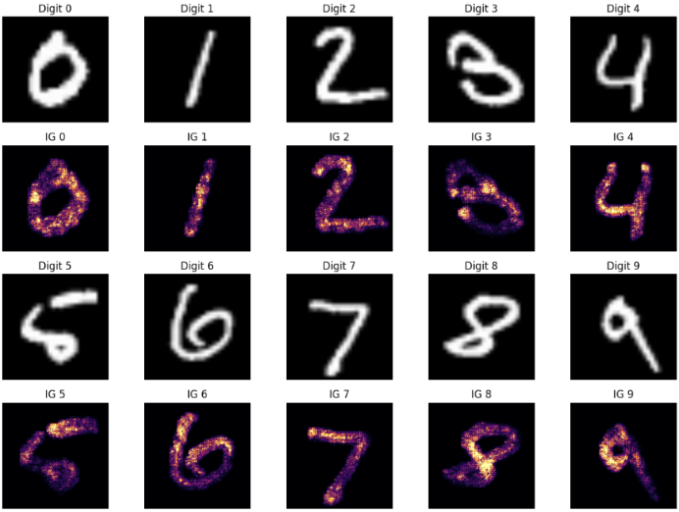
\includegraphics[width=0.8\textwidth]{imgs/mnist_ig_clean.png}
    \caption{Mapy atrybucji dla obrazów niezaszumionych}
    \label{fig:mnist_ig_clean}
\end{figure}
\noindent Na rysunku zauważyć można, że dla analizowanych cyfr najwyższe wartości atrybucji koncentrowały się w obszarach odpowiadających właściwemu kształtowi liczby skupiając się na kluczowych dla każdej cyfry elementach geometrii, takich jak charakterystyczne zaokrąglenia, przecięcia linii czy punkty zwrotne. W przypadku cyfr o zamkniętych pętlach, takich jak 0, 6, 8 czy 9, model wyraźnie zaznacza ich obwody, co pozwala mu skutecznie odróżnić te cyfry od siebie nawzajem oraz od bardziej liniowych konstrukcji. Podobnie w sytuacjach, gdzie kluczowe znaczenie ma przecięcie linii, jak ma to miejsce w cyfrach 2, 4 czy 7, mapy atrybucji wskazują precyzyjnie na te krytyczne złącza, potwierdzając, że stanowią one najważniejszą informację dla podjęcia decyzji klasyfikacyjnej. W przypadku obrazów MNIST taka interpretacja jest szczególnie czytelna, ponieważ tło obrazu jest jednorodne, a najważniejsza informacja wizualna znajduje się w obrębie samej cyfry.

Mapy Integrated Gradients dla obrazów niezaburzonych stanowiły punkt odniesienia dla dalszej analizy stabilności. W kolejnym kroku zbadano mapy atrybucji przykładów niezaszumionych z zaszumionymi. Porównanie przedstawiono na rysunku \ref{fig:mnist_ig_sg_vs_clean}.
\begin{figure}[H]
    \centering
    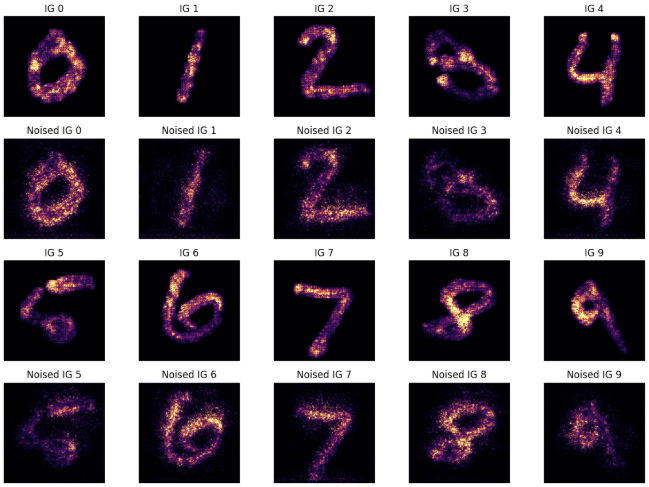
\includegraphics[width=0.8\textwidth]{imgs/mnist_ig_sg_vs_clean.png}
    \caption{Porównanie map atrybucji obrazów niezaszumionych i zaszumionych}
    \label{fig:mnist_ig_sg_vs_clean}
\end{figure}
\noindent Po dodaniu szumu Gaussa mapy atrybucji zachowywały częściową zgodność z mapami uzyskanymi dla obrazów oryginalnych. Najważniejsze obszary nadal znajdowały się w pobliżu kształtu cyfry, jednak atrybucje stawały się bardziej rozproszone. Widoczne były również dodatkowe aktywacje poza właściwym obszarem cyfry, co wskazuje, że zakłócenia tła wpływały na sposób wyznaczania istotności przez metodę Integrated Gradients.

W celu zweryfikowania tych obserwacji przeprowadzono analizę ilościową. Dla kolejnych poziomów szumu porównano mapy atrybucji obrazów oryginalnych i zaburzonych za pomocą podobieństwa cosinusowego oraz metryki Top-K IoU. Pozwoliło to ocenić, w jakim stopniu zmiany widoczne na mapach przekładały się na mierzalny spadek stabilności wyjaśnień. Wartości metryk przedstawiono w tabeli \ref{tab:ig_sg_cos_topk_mnist}.

\begin{table}[H]
    \centering
    \caption{Zestawienie metryk podobieństwa dla różnych wartości parametru \(\sigma\) dla zbioru MNIST i metody Integrated Gradients}
    \label{tab:ig_sg_cos_topk_mnist}
    \begin{tabular}{ccccc}
    \toprule
    $\sigma$ & $\overline{cos}$ & $SD_{cos}$ & $\overline{IoU}_{K}$ & $SD_{IoU}$ \\
    \midrule
    0.010 & 0.901 & 0.026 & 0.764 & 0.078 \\
    0.030 & 0.839 & 0.025 & 0.681 & 0.087 \\
    0.050 & 0.813 & 0.022 & 0.646 & 0.088 \\
    0.075 & 0.793 & 0.022 & 0.619 & 0.086 \\
    0.100 & 0.780 & 0.022 & 0.600 & 0.085 \\
    0.150 & 0.758 & 0.018 & 0.574 & 0.081 \\
    0.200 & 0.736 & 0.020 & 0.553 & 0.079 \\
    0.300 & 0.709 & 0.023 & 0.519 & 0.073 \\
    0.500 & 0.659 & 0.033 & 0.465 & 0.065 \\
    0.800 & 0.598 & 0.036 & 0.400 & 0.057 \\
    \bottomrule
    \end{tabular}
\end{table}

\noindent Wyniki pokazują systematyczny spadek stabilności wyjaśnień wraz ze wzrostem wartości parametru $\sigma$. Dla najmniejszego poziomu szumu, $\sigma$ = 0{,}010, średnie podobieństwo cosinusowe wynosiło (0{,}901), natomiast średnia wartość Top-K IoU była równa 0{,}764. Oznacza to, że przy bardzo słabym zakłóceniu mapy atrybucji pozostawały w dużym stopniu zgodne z mapami uzyskanymi dla obrazów oryginalnych. Wraz ze wzrostem intensywności szumu obie metryki stopniowo malały. Dla największej analizowanej wartości, $\sigma$ = 0{,}800, podobieństwo cosinusowe spadło do 0{,}598, a Top-K IoU do 0{,}400. Spadek podobieństwa cosinusowego wskazuje, że ogólny rozkład wartości atrybucji stawał się coraz mniej zbliżony do rozkładu uzyskanego dla obrazów niezaburzonych. Jednocześnie spadek Top-K IoU oznacza, że zmieniało się również położenie najbardziej istotnych pikseli. Odchylenia standardowe dla podobieństwa cosinusowego były stosunkowo niewielkie i mieściły się w przedziale od 0{,}018 do 0{,}036, co wskazuje na dość spójny trend spadkowy w analizowanych przykładach. W przypadku Top-K IoU odchylenia standardowe również nie były wysokie, a ich wartości stopniowo malały dla większych poziomów szumu. Może to oznaczać, że przy silniejszych perturbacjach spadek zgodności najważniejszych obszarów był bardziej jednolity dla różnych cyfr.

Po zbadaniu metryk podobieństwa przystąpiono do analizy metryki Deletion AUC w celu sprawdzenia, jak usuwanie pikseli wskazanych przez mapę atrybucji jako istotne wpływało na pewność modelu względem analizowanej klasy. Dzięki temu możliwe było uzupełnienie wcześniejszej oceny stabilności o informację, czy obszary wyróżniane przez metodę Integrated Gradients rzeczywiście miały znaczenie dla decyzji klasyfikacyjnej. Wyniki dla kolejnych wartości parametru $\sigma$ przedstawiono w tabeli \ref{tab:gaussian_noise_auc_conf_mnist}.

\begin{table}[H]
    \centering
    \caption{Wpływ wartości szumu Gaussa na metryki AUC, pewność predykcji oraz liczbę zmian predykcji}
    \label{tab:gaussian_noise_auc_conf_mnist}
    \begin{tabular}{cccccccc}
    \toprule
    $\sigma$ &
    $\overline{AUC}_{c}$ &
    $SD_{AUC,c}$ &
    $\overline{AUC}_{p}$ &
    $SD_{AUC,p}$ &
    $\overline{Conf}_{c}$ &
    $\overline{Conf}_{p}$ &
    $N_{chg}$ \\
    \midrule
    0.010 & 0.279 & 0.236 & 0.411 & 0.276 & 0.997 & 0.997 & 0 \\
    0.030 & 0.279 & 0.236 & 0.381 & 0.266 & 0.997 & 0.996 & 0 \\
    0.050 & 0.279 & 0.236 & 0.328 & 0.274 & 0.997 & 0.995 & 0 \\
    0.075 & 0.279 & 0.236 & 0.287 & 0.281 & 0.997 & 0.994 & 0 \\
    0.100 & 0.279 & 0.236 & 0.241 & 0.267 & 0.997 & 0.991 & 1 \\
    0.150 & 0.279 & 0.236 & 0.203 & 0.256 & 0.997 & 0.986 & 1 \\
    0.200 & 0.279 & 0.236 & 0.171 & 0.235 & 0.997 & 0.981 & 1 \\
    0.300 & 0.279 & 0.236 & 0.145 & 0.222 & 0.997 & 0.961 & 3 \\
    0.500 & 0.279 & 0.236 & 0.121 & 0.200 & 0.997 & 0.905 & 7 \\
    0.800 & 0.279 & 0.236 & 0.104 & 0.172 & 0.997 & 0.703 & 24 \\
    \bottomrule
    \end{tabular}   
\end{table}

\noindent Wartości $\overline{AUC}{c}$ oraz $\overline{Conf}{c}$ pozostają stałe dla wszystkich poziomów szumu, ponieważ odnoszą się do tych samych obrazów niezaburzonych, które stanowiły punkt odniesienia w eksperymencie. Średnia wartość Deletion AUC dla obrazów oryginalnych wyniosła 0{,}279, natomiast średnia pewność modelu względem klasy docelowej była bardzo wysoka i wynosiła 0{,}997. Dla obrazów zaburzonych można zauważyć wyraźną zmianę wartości Deletion AUC wraz ze wzrostem parametru $\sigma$. Przy najmniejszym poziomie szumu, $\sigma = 0{,}010$, średnia wartość $\overline{AUC}_{p}$ wynosiła 0{,}411, a więc była wyższa niż dla obrazów oryginalnych. Następnie wartość ta systematycznie malała, osiągając 0{,}241 dla $\sigma = 0{,}100$, 0{,}145 dla $\sigma = 0{,}300$ oraz 0{,}104 dla największego poziomu szumu, $\sigma = 0{,}800$. Oznacza to, że wraz ze wzrostem intensywności zakłócenia zmieniał się wpływ usuwania pikseli wskazanych przez mapę atrybucji na pewność modelu. Interpretując te wyniki, należy uwzględnić również średnią pewność modelu dla obrazów zaburzonych. Dla małych wartości $\sigma$ pozostawała ona bardzo wysoka i zbliżona do wartości uzyskanej dla obrazów oryginalnych. Przykładowo dla $\sigma = 0{,}010$ wynosiła 0{,}997, a dla $\sigma = 0{,}100$ nadal utrzymywała się na poziomie 0{,}991. Oznacza to, że niewielki szum nie zaburzał istotnie decyzji modelu. Dopiero dla większych wartości parametru widoczny był wyraźniejszy spadek pewności, szczególnie dla $\sigma = 0{,}500$, gdzie wyniosła ona 0{,}905, oraz dla $\sigma = 0{,}800$, gdzie spadła do 0{,}703. Wraz ze wzrostem poziomu szumu rosła także liczba przypadków, w których predykcja modelu uległa zmianie. Dla wartości $\sigma$ do 0{,}075 nie odnotowano żadnych zmian predykcji, natomiast dla $\sigma = 0{,}100$ pojawiła się pierwsza taka zmiana. Przy silniejszych perturbacjach liczba zmian wzrastała, osiągając 7 przypadków dla $\sigma = 0{,}500$ oraz 24 przypadki dla $\sigma = 0{,}800$. Pokazuje to, że przy największych poziomach szumu wyniki Deletion AUC należy interpretować ostrożnie, ponieważ są one powiązane nie tylko z właściwościami map atrybucji, ale również z pogorszeniem stabilności samej klasyfikacji.

\section{Wpływ ataku FGSM na wyjaśnienia generowane metodą Integrated Gradients}
\label{sec:ig_vs_fgsm_mnist}

Przystąpiono do analizy wpływu ataku FGSM na wyjaśnienia generowane metodą Integrated Gradients. Tak jak w poprzednim eksperymencie, punktem odniesienia były mapy atrybucji wyznaczone dla obrazów niezaburzonych. Porównanie map atrybucji przedstawiono na rysunku \ref{fig:mnist_ig_fgsm_vs_clean}.

\begin{figure}[H]
    \centering
    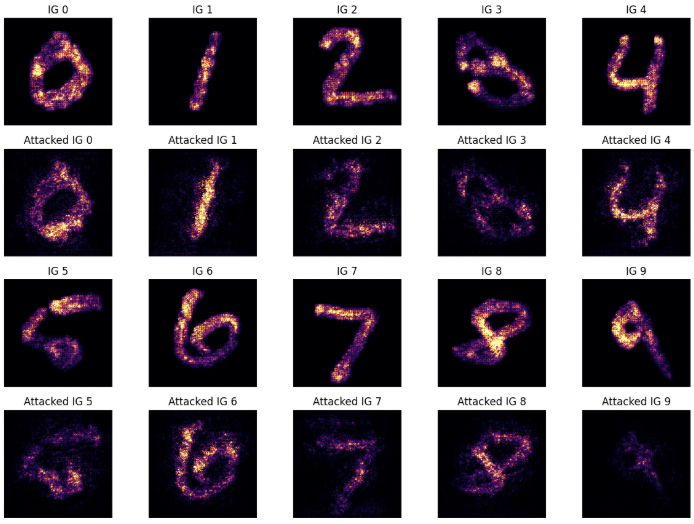
\includegraphics[width=0.8\textwidth]{imgs/mnist_ig_fgsm_vs_clean.png}
    \caption{Porównanie map atrybucji obrazów niezaatakowanych i zaatakowanych}
    \label{fig:mnist_ig_fgsm_vs_clean}
\end{figure}

\noindent Po zastosowaniu ataku FGSM mapy atrybucji uległy zauważalnym zmianom względem map otrzymanych dla obrazów oryginalnych. W wielu przypadkach główny zarys cyfry pozostawał jeszcze widoczny, jednak atrybucje były mniej zwarte i bardziej rozproszone. Tutaj {-} w przeciwieństwie do szumu Gaussa {-} szczególnie widoczne były osłabienia fragmentów, które wcześniej tworzyły wyraźny kształt cyfr. Mapy po ataku stały się wyraźnie mniej czytelna i trudniej było wskazać jednoznaczny obszar odpowiedzialny za decyzję modelu. Zauważono również pojedyncze aktywacje w tle poza geometrią cyfr.

W tabeli \ref{tab:ig_fgsm_cos_topk_mnist} pokazano wyniki metryk dla map atrybucji po zastosowaniu ataku FGSM na obrazach wejściowych dla różnych wartości $\epsilon$.
\begin{table}[H]
    \centering 
    \caption{Zestawienie metryk podobieństwa dla różnych wartości parametru \(\epsilon\) dla zbioru MNIST i metody Integrated Gradients} 
    \label{tab:ig_fgsm_cos_topk_mnist} 
    \begin{tabular}{ccccc} 
    \toprule $\epsilon$ & $\overline{cos}$ & $SD_{cos}$ & $\overline{IoU}_{K}$ & $SD_{IoU}$ \\ 
    \midrule 
    0.010 & 0.853 & 0.023 & 0.707 & 0.090 \\
    0.030 & 0.801 & 0.020 & 0.638 & 0.097 \\
    0.050 & 0.777 & 0.021 & 0.610 & 0.095 \\ 
    0.075 & 0.755 & 0.024 & 0.584 & 0.093 \\
    0.100 & 0.736 & 0.028 & 0.564 & 0.091 \\
    0.150 & 0.701 & 0.034 & 0.534 & 0.089 \\ 
    0.200 & 0.672 & 0.039 & 0.510 & 0.086 \\ 
    0.300 & 0.623 & 0.049 & 0.466 & 0.082 \\ 
    0.400 & 0.579 & 0.060 & 0.426 & 0.083 \\
    0.500 & 0.541 & 0.067 & 0.390 & 0.083 \\ 
    \bottomrule 
    \end{tabular} 
\end{table}

\noindent Wyniki z tabeli \ref{tab:ig_fgsm_cos_topk_mnist} wskazują na systematyczny spadek zgodności map wraz ze wzrostem wartości parametru $\epsilon$. Dla najmniejszej wartości perturbacji $\epsilon = 0{,}010$ średnie podobieństwo cosinusowe wynosiło $0{,}853$, a średnia wartość Top-K IoU $0{,}707$. Oznacza to, że nawet przy niewielkiej wartości parametru $\epsilon$ mapy atrybucji po ataku różniły się zauważalnie od map uzyskanych dla obrazów oryginalnych. Wraz ze wzrostem siły ataku obie metryki stopniowo malały. Dla największej analizowanej wartości $\epsilon = 0{,}500$ podobieństwo cosinusowe spadło do $0{,}541$, natomiast Top-K IoU do $0{,}390$. Spadek podobieństwa cosinusowego wskazuje, że ogólny rozkład atrybucji stawał się coraz mniej podobny do rozkładu uzyskanego dla obrazów niezaburzonych. Jednocześnie obniżenie wartości Top-K IoU oznacza, że zmieniało się położenie pikseli uznawanych przez metodę za najistotniejsze. Odchylenia standardowe dla podobieństwa cosinusowego rosły wraz ze wzrostem wartości $\epsilon$, od $0{,}023$ dla $\epsilon = 0{,}010$ do $0{,}067$ dla $\epsilon = 0{,}500$. Może to wskazywać, że silniejsze perturbacje wpływały na poszczególne przykłady w bardziej zróżnicowany sposób. W przypadku Top-K IoU odchylenia standardowe pozostawały na zbliżonym poziomie, co sugeruje, że spadek zgodności najważniejszych obszarów był względnie konsekwentny w całym analizowanym zbiorze przykładów.

Tabela \ref{tab:ig_fgsm_auc_conf_mnist} przedstawia wartości metryki Deletion AUC dla ataku FGSM przy różnych wrtościach $\epsilon$.

\begin{table}[H] \centering \caption{Wpływ wartości parametru \(\epsilon\) ataku FGSM na metryki AUC, pewność predykcji oraz liczbę zmian predykcji dla zbioru MNIST i metody Integrated Gradients}  \label{tab:ig_fgsm_auc_conf_mnist} \begin{tabular}{cccccccc} \toprule $\epsilon$ & $\overline{AUC}_{c}$ & $SD_{AUC,c}$ & $\overline{AUC}_{p}$ & $SD_{AUC,p}$ & $\overline{Conf}_{c}$ & $\overline{Conf}_{p}$ & $N_{chg}$ \\ \midrule 0.010 & 0.279 & 0.236 & 0.369 & 0.264 & 0.997 & 0.993 & 0 \\ 0.030 & 0.279 & 0.236 & 0.302 & 0.258 & 0.997 & 0.977 & 2 \\ 0.050 & 0.279 & 0.236 & 0.231 & 0.240 & 0.997 & 0.955 & 4 \\ 0.075 & 0.279 & 0.236 & 0.171 & 0.207 & 0.997 & 0.918 & 7 \\ 0.100 & 0.279 & 0.236 & 0.136 & 0.180 & 0.997 & 0.879 & 9 \\ 0.150 & 0.279 & 0.236 & 0.105 & 0.144 & 0.997 & 0.778 & 18 \\ 0.200 & 0.279 & 0.236 & 0.088 & 0.122 & 0.997 & 0.630 & 33 \\ 0.300 & 0.279 & 0.236 & 0.067 & 0.087 & 0.997 & 0.391 & 56 \\ 0.400 & 0.279 & 0.236 & 0.055 & 0.065 & 0.997 & 0.244 & 74 \\ 0.500 & 0.279 & 0.236 & 0.047 & 0.056 & 0.997 & 0.167 & 83 \\ \bottomrule \end{tabular} \end{table}

\noindent Dla obrazów po zastosowaniu FGSM widoczny jest wyraźny spadek wartości $\overline{AUC}{p}$ wraz ze wzrostem parametru $\epsilon$. Dla najmniejszej wartości $\epsilon = 0{,}010$ średnia wartość Deletion AUC wynosiła $0{,}369$, natomiast dla $\epsilon = 0{,}050$ spadła do $0{,}231$. Przy dalszym zwiększaniu siły ataku spadek był jeszcze bardziej widoczny: dla $\epsilon = 0{,}200$ wartość $\overline{AUC}{p}$ wyniosła $0{,}088$, a dla największej analizowanej wartości $\epsilon = 0{,}500$ jedynie $0{,}047$. Dla małych wartości $\epsilon$ model nadal zachowywał wysoką pewność względem klasy docelowej. Przykładowo dla $\epsilon = 0{,}010$ średnia pewność wynosiła $0{,}993$, a predykcja nie zmieniła się ani razu. Jednak już dla $\epsilon = 0{,}030$ pojawiły się 2 zmiany predykcji, a pewność spadła do $0{,}977$. Oznacza to, że nawet niewielka perturbacja FGSM zaczynała wpływać na decyzje modelu. Dla większych wartości $\epsilon$ wpływ ataku był znacznie silniejszy. Średnia pewność modelu spadła z $0{,}879$ dla $\epsilon = 0{,}100$ do $0{,}630$ dla $\epsilon = 0{,}200$, a następnie do $0{,}167$ dla $\epsilon = 0{,}500$. Równocześnie liczba zmienionych predykcji wzrosła z 9 dla $\epsilon = 0{,}100$ do 33 dla $\epsilon = 0{,}200$ oraz 83 dla $\epsilon = 0{,}500$. Tak duży wzrost liczby zmian predykcji pokazuje, że dla wysokich wartości $\epsilon$ atak FGSM znacząco zaburzał działanie modelu klasyfikacyjnego.


\section{Wpływ szumu Gaussa na wyjaśnienia generowane metodą Occlusion}
\label{sec:occ_vs_szum_gaussa_mnist}

\section{Wpływ ataku FGSM na wyjaśnienia generowane metodą Occlusion}
\label{sec:occ_vs_fgsm_mnist}